\section{Justificação da Arquitetura Adotada}

Na Figura \ref{fig:diagrama_arquitetura} está representada a arquitetura da aplicação desenvolvida no AWS, e como é possível visualizar, ela encontra-se devidida nas duas principais camadas: o frontend e o backend.

\begin{figure}[h]
	\centering
	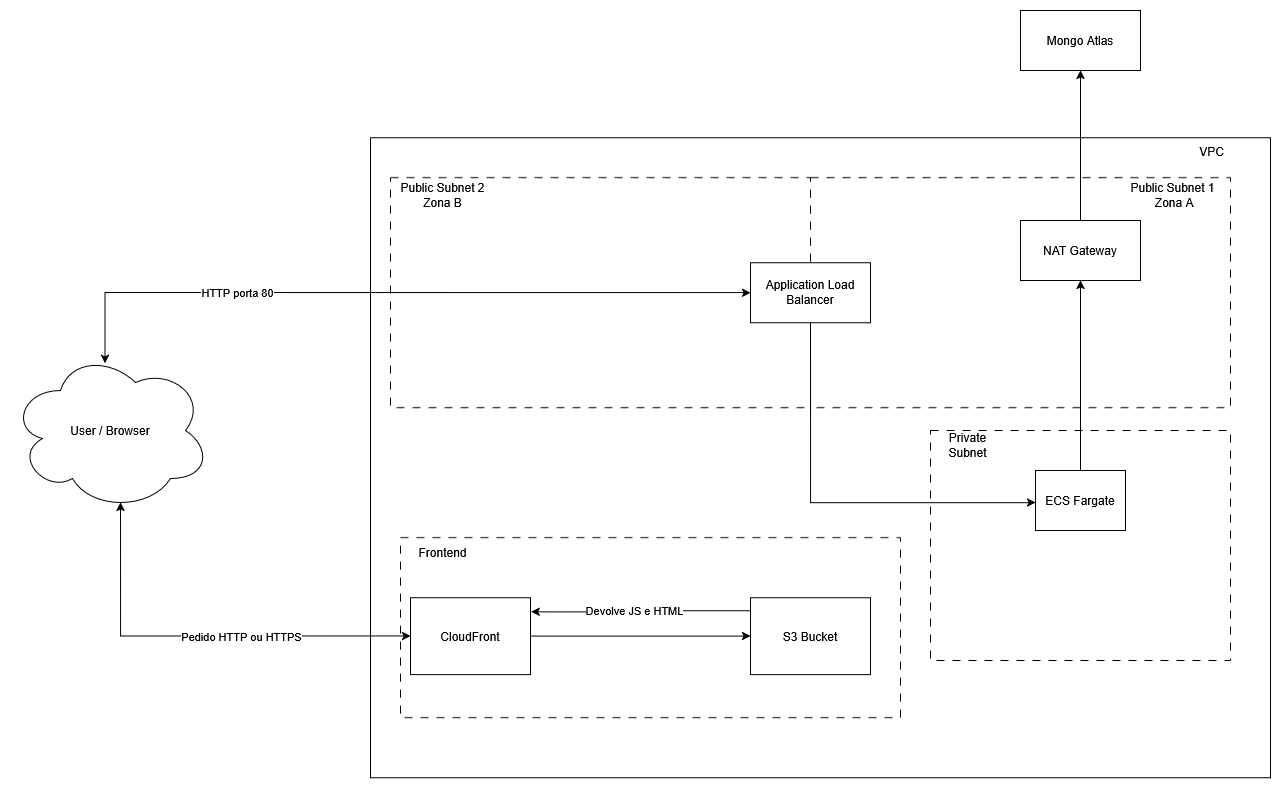
\includegraphics[width=0.8\linewidth]{imagens/Diagrama_CDN}
	\caption{Diagrama de Arquitetura}
	\label{fig:diagrama_arquitetura}
\end{figure}

\begin{itemize} 
	\item \textbf{Frontend:} Este está num \textit{bucket} S3 privado e acessível via Amazon CloudFront (CDN).
	
	\item \textbf{Backend:} Este está implementado numa VPC (\textit{Virtual Private Cloud}) segmentada. A API executa sobre Amazon ECS com Fargate, estando numa subnet privada de modo a estar totalmente isolada da internet. O tráfego de entrada é gerido por um \textit{Application Load Balancer} (ALB) localizado nas duas subnets públicas, e está responsável por encaminhar os pedidos para os containers.
\end{itemize}

O backend comunica com uma base de dados MongoDB, mas esta não existe dentro do AWS, mas sim como um serviço externo, o MongoDB Atlas, portanto o URI de conexão ao mesmo é passado como uma variável de ambiente na configuração do Open Tofu. Estando depois disponível à API através do intermédio da NAT Gateway, que é necessário visto que a API encontra-se numa subnet privada.
